\documentclass[12pt]{article}
\usepackage{amsfonts, amssymb, amsmath, amsthm}
\usepackage[margin=1in]{geometry}
\usepackage{tikz}

\title{Explainer: Problem 7 (Rudin 7.5) --- Disjoint Bumps: Absolute but Not Uniform Convergence}
\author{}
\date{}

\begin{document}
\maketitle

\section*{The sequence}
$$
f_n(x) = \begin{cases}
\sin^2(\pi/x) & \text{if } \frac{1}{n+1} \leq x \leq \frac{1}{n}, \\
0 & \text{otherwise}.
\end{cases}
$$
Each $f_n$ is a bump supported on the tiny interval $\left[\frac{1}{n+1}, \frac{1}{n}\right]$.

\begin{center}
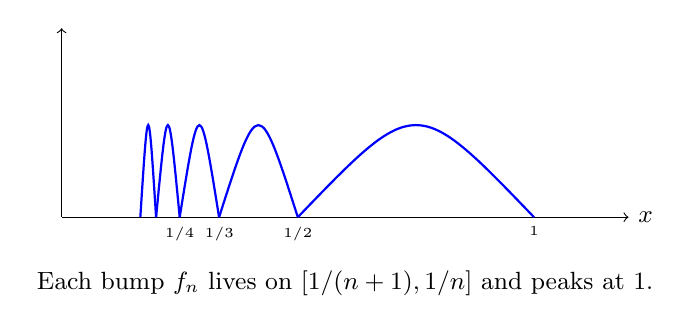
\begin{tikzpicture}[scale=1.2]
  \draw[->] (0, 0) -- (6, 0) node[right] {\small $x$};
  \draw[->] (0, 0) -- (0, 2);
  \foreach \n in {1,2,3,4,5} {
    \pgfmathsetmacro\a{5/(\n+1)}
    \pgfmathsetmacro\b{5/\n}
    \pgfmathsetmacro\mid{(\a+\b)/2}
    \draw[thick, blue] (\a, 0) .. controls (\mid, 1.3) .. (\b, 0);
  }
  \node[below] at (5, 0) {\tiny $1$};
  \node[below] at (2.5, 0) {\tiny $1/2$};
  \node[below] at (1.67, 0) {\tiny $1/3$};
  \node[below] at (1.25, 0) {\tiny $1/4$};
  \node at (3, -0.7) {\small Each bump $f_n$ lives on $[1/(n+1), 1/n]$ and peaks at $1$.};
\end{tikzpicture}
\end{center}

\section*{Two claims}
\begin{enumerate}
  \item $\{f_n\}$ converges pointwise to a \textbf{continuous} function (it's the zero function), but not uniformly.
  \item The series $\sum f_n$ converges absolutely for every $x$, but not uniformly.
\end{enumerate}

\section*{Why pointwise $\to 0$}
Fix any $x \in \mathbb{R}$.
\begin{itemize}
  \item If $x \leq 0$: every $f_n(x) = 0$.
  \item If $x > 1$: also $0$ for all $n \geq 1$.
  \item If $0 < x \leq 1$: $x$ lies in at most one interval $[1/(n+1), 1/n]$, so $f_n(x) \neq 0$ for only \emph{one} value of $n$; for all larger $n$, $f_n(x) = 0$.
\end{itemize}
So $f_n(x) \to 0$ for every $x$. The limit function is identically $0$ --- continuous.

\section*{Why NOT uniformly}
The bumps all reach height $1$ (take $x$ where $\pi/x = \pi/2$, i.e., $x = 2$... wait, you need this inside the bump support). In each bump interval $[1/(n+1), 1/n]$, does $\sin^2(\pi/x)$ attain the value $1$?

Yes: $\sin^2(\pi/x) = 1$ when $\pi/x = \pi/2 + k\pi$, i.e., $x = 2/(2k+1)$. For each $n$, you can find such a $k$ making $x$ lie in $[1/(n+1), 1/n]$ (since the interval is large enough to contain one of these points for big $n$).

So $\sup_x f_n(x) = 1$ for every $n$, which doesn't go to $0$. Not uniform.

\section*{The series $\sum f_n$}
At each $x$, at most \emph{one} $f_n(x) \neq 0$. So the series is essentially a single term at every $x$ --- \textbf{absolutely convergent} (trivially).

\textbf{But not uniformly:} The partial sum $S_N(x) = \sum_{n=1}^{N} f_n(x)$ differs from the full sum by $\sum_{n > N} f_n$, which is \emph{nonzero} on $(0, 1/(N+1)]$ and still reaches height $1$. So $\sup |S - S_N|$ doesn't $\to 0$.

\section*{Takeaway}
\textbf{Absolute pointwise convergence is much weaker than uniform convergence.} Even when each $x$ sees only one nonzero term (so absolute convergence is automatic), the \emph{location} of the nonzero term can shift, keeping the worst-case error bounded away from $0$.

\end{document}
